\chapter{Automated Decryption}

As article {\it Inductive programming meets the real world} \cite{Gulwani2015} states, that we should try to automate everything we can in order to avoid repetitive tasks.
Even though disc encryption provides another layer of security to our data, it is used less.
Typing one more pass-phrase when accessing some removable storage seems like too much work.
More crucial would be full disk encryption.
In order to boot the system, we need to have storage with system decrypted -- provide another pass-phrase every time the computer is turned off and on again.
The Tang server aims to solve struggles with the early boot decryption of system volumes.
Before Tang, automated decryption was usually handled by a Key Escrow server.

\section{Key Escrow}\label{escrow}

The Key Escrow server (also known as a “fair” cryptosystem) is providing escrow service for encryption keys.
A client using Key Escrow usually generates a key, encrypts data with it and then stores the key encryption key on a remote server.
Unfortunately there are couple of security concerns.

To transfer the encryption keys we want to store on an Escrow server, we have to encrypt the channel on which we send them.
When transmitting keys over an insecure network without an encrypted link, anyone listening to the network traffic could immediately fetch the key.
This should signal security risks, and, of course, we do not want any third party to access our secret data.
Usually we encrypt a channel with TLS (Transport Layer Security) or GSSAPI (Generic Security Services Application Program Interface) as shown on a Figure \ref{fig_escrowmodel} Escrow model.
\begin{figure}[h]
    \centering
    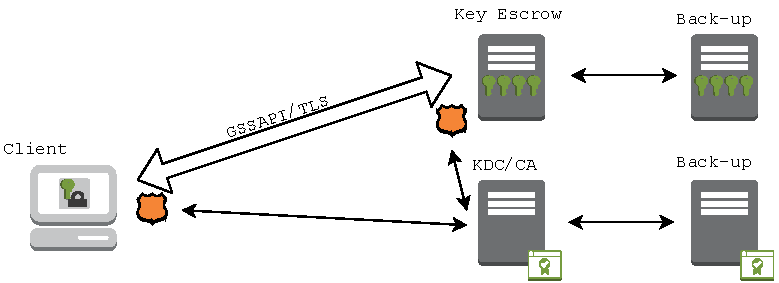
\includegraphics[scale=0.7]{figures/EscrowModel.pdf}
    \caption{Escrow Model}
    \label{fig_escrowmodel}
\end{figure}
Unfortunately, this is not enough to have the communication secure.
This server has to have its identity verified, and the client has to authenticate to this server too.
The increasing amount of keys implicates a need for Certification Authority server (CA) or a Key Distribution Center (KDC) to manage all of them.

Only with the infrastructure in place and keys produced, the server can verify if the client is permitted to get their key, and the client is able to identify a trusted server.
This is a fully stateful process.

The complexity of this system increases the attack surface and for such complex system it would be unimaginable not to have backups.
The Escrow server may store lots of keys from lots of different places, users and services.



\section{Tang Server}\label{tang}

With key escrow, a third party gets copies of a cryptographic key.
People might not be comfortable with any third party having this ability and that “technical” problems vex the key escrow solution.
Tang's key recovery, on the other hand, lets us just “backup” and restore cryptographic keys anonymously and without any third party possesing our key.

Tang is a very lightweight network service using systemd's socket activation as described in section \ref{socket_activation}.
Its purpose is to provide anonymous key recovery to clients over the network.
This key recovery can be used with a help of the Tang's client descibed in subsection \ref{clevis} Clevis client to unlock data storages with LUKS encryption.
The Tang server is an open source project implemented in C programming language.

We can see on Figure \ref{fig_tangmodel} that the Tang model is very similar to the escrow seen on Figure \ref{fig_escrowmodel} but with some things missing.
\begin{figure}[h]
    \centering
    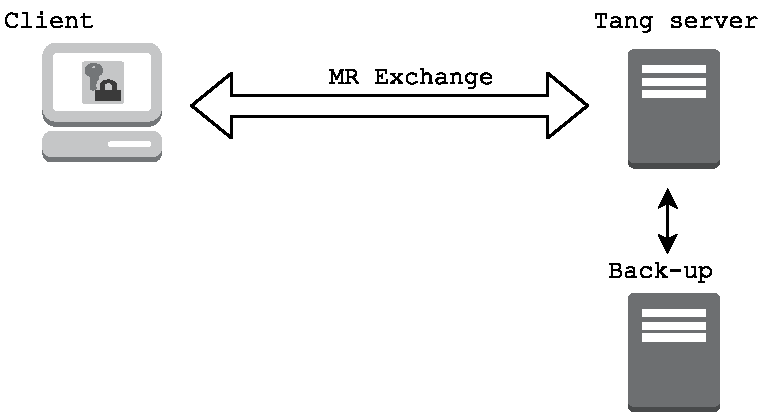
\includegraphics[scale=0.7]{figures/TangModel.pdf}
    \caption{Tang Model}
    \label{fig_tangmodel}
\end{figure}
In fact, there is no longer need for TLS channel to secure communication between the client and the server,
 and that is because Tang implements the McCallum-Relyea exchange as described below.

Tang server advertises asymmetric keys on the network and a client is able to get the list of these signing keys by HTTP (Hypertext Transfer Protocol) GET request.
All tang communication is performed using the HTTP protocol with the message body in JWK (JSON Web Key) format defined by RFC 7517 \cite{RFC7517}.
Getting advertised keys is the first step of the McCallum-Relyea exchange protocol summed up in table \ref{mrexchange}.
\begin{table}[h]
\centering
\label{mrexchange}
\begin{tabular}{c|c|c|c}
\hline
\multicolumn{2}{c|}{Provisioning} & \multicolumn{2}{c}{Recovery} \\ \hline
client's side & server's side & client's side & server's side \\ \hline
 & $ S \epsilon _{bindingR} [1, p-1]$ & $E \epsilon _{R} [1, p-1]$ &  \\
 & $s = g * S$ &$ x = c + g * E$ &  \\
\multicolumn{2}{c|} {$\leftarrow$  s} & \multicolumn{2}{c} {x $\rightarrow$}  \\
$C \epsilon _{R} [1, p-1]$ &  &  & $y = z * S$\\
$e = g * C $&  & \multicolumn{2}{c} {$\leftarrow$ y} \\
$k = g * S * C = s * C$ &  & $k = y - s * E$&  \\
Discard: K, C &  &  &  \\
Retain s, c &  &  &  \\ \hline
\multicolumn{4}{c}{*capital is private key; g stands for generate}
\end{tabular}
\caption{McCallum-Relyea Exchange Protocol}
\end{table}
This protocol has two phases, provisioning and recovery.

\paragraph{Provisioning}
The server key pair generation is represented by equation \ref{servergen}, capital is private key; lowercase is public key; g stands for generate.
\begin{equation}\label{servergen}
    s = g * S
\end{equation}
After the server generates key pair, it is advertising the public part of it.
The client then selects one of the Tang server's exchange keys (we will call it {\it sJWK}; identified by the use of {\it deriveKey} in the {\it sJWK}'s {\it key\_ops} attribute).
The lowercase “s” stands for server's public key and JWK is format of the message.
The client then generates a new (random) JWK ({\it cJWK}; c stands for client's key pair).
\begin{equation}\label{clientgen}
    c = g * C
\end{equation}
The client performs its half of a standard ECDH exchange producing {\it kJWK} -- see equation \ref{kJWK_gen}, which it uses to encrypt the data.
Afterwards, it must discard the {\it kJWK} and the private key from {\it cJWK}.
\begin{equation}\label{kJWK_gen}
    k = s * C
\end{equation}
The client has to store {\it cJWK} for later use in the recovery step.
Generally speaking, the client may also store other data, such as the URL of the Tang server or the trusted advertisement signing keys called also binding keys.



\paragraph{Recovery}
Mathematically capital letter is private key; g stands for generate.
When the client wants to access the encrypted data, it must be able to recover encryption key.
To recover {\it kJWK} after discarding it, the client generates a third ephemeral key ({\it eJWK}) as the equation \ref{eqn_ephemeral} represent.
This key is used to hide the client's public key and the binding key.
\begin{equation}\label{eqn_ephemeral}
    e = g * E
\end{equation}
The ephemeral key is generated for each execution of a key establishment process.
Using {\it eJWK}, the client performs elliptic curve group addition of {\it eJWK} and {\it cJWK}, producing {\it xJWK} represented in the equation \ref{eqn_ecga}.
The client {\it POST}s {\it xJWK} to the server.
\begin{equation}\label{eqn_ecga}
    x = c + e
\end{equation}
The server then performs its half of the ECDH key exchange using {\it xJWK} and {\it sJWK}, producing {\it yJWK} reflected in the equation \ref{eqn_response}. The server returns {\it yJWK} to the client.
\begin{equation}\label{eqn_response}
    y = x * S
\end{equation}
The client then performs half of an ECDH key exchange between {\it eJWK} and {\it sJWK}, producing {\it zJWK} as the equation \ref{eqn_get} shows.
\begin{equation}\label{eqn_get}
    z = s * E
\end{equation}
Subtracting {\it zJWK} from {\it yJWK} produces {\it dJWK} shown in the equation \ref{eqn_extract}.
\begin{equation}\label{eqn_extract}
    k = y - z
\end{equation}
Finally, the client has calculated the key value.
So the Tang server never knows the value of the key and literally nothing about its clients.



\subsection{Security}

As shown in table \ref{compare}, Tang compared to Escrow is stateless and doesn't require TLS or authentication.
Tang also has limited knowledge.
Unlike escrows, where the server has knowledge of every key used, Tang never sees any client keys.
Tang never gains any identifying information from the client.

\begin{table}[h]
\centering
\label{compare}
\begin{tabular}{@{}lll@{}}
\toprule
               & Escrow   & Tang                         \\ \midrule
Stateless      & No       & Yes                          \\
SSL/TLS        & Required & Optional                     \\
X.509          & Required & Optional                     \\
Authentication & Required & Optional                     \\
Anonymous      & No       & Yes                          \\ \bottomrule
\end{tabular}
\caption{Comparing Escrow and Tang}
\end{table}

Thanks to McCallum-Relyea exchange protocol summed up in the table \ref{mrexchange} Tang is resistant to the man in the middle attack.
In case of the eavesdroppers, they see the client send {\it xJWK} and receive {\it yJWK}.
Since these packets are blinded by {\it eJWK}, only the party that can un-blind these values is the client itself (since only it has {\it eJWK}'s private key).
Thus, the attack fails.

It is of utmost importance that the client protects {\it cJWK} and the Tang server must protect the private key for {\it sJWK}.



\subsection{Building Tang}

Tang is originally packaged for Fedora operating system version 23 and later but we can of course build it from source.
It relies on few other software libraries listed in section \ref{dependencies}.

The steps to build the Tang from sources include downloading the source from project's GitHub or cloning~it.
Make sure all required dependencies are installed and then run:
\begin{lstlisting}[columns=fixed,basicstyle=\ttfamily\footnotesize,tabsize=4,backgroundcolor=\color{yellow!10}]
$ autoreconf -if
$ ./configure --prefix=/usr
$ make
# make install
\end{lstlisting}
Optionally tests can be run with:
\begin{lstlisting}[columns=fixed,basicstyle=\ttfamily\footnotesize,tabsize=4,backgroundcolor=\color{yellow!10}]
$ make check
\end{lstlisting}



\subsection{Server Enablement}

Enabling a Tang server is a two-step process.
First step is to enable the Tang services.
Start the key update service which is watching the database directory using systemd:
\begin{lstlisting}[columns=fixed,basicstyle=\ttfamily\footnotesize,tabsize=4,backgroundcolor=\color{yellow!10}]
# systemctl enable tangd-update.path --now
\end{lstlisting}
Enable service using systemd socket activation:
\begin{lstlisting}[columns=fixed,basicstyle=\ttfamily\footnotesize,tabsize=4,backgroundcolor=\color{yellow!10}]
# systemctl enable tangd.socket --now
\end{lstlisting}
After this, systemd will handle the sockets and the Tang's key rotation procedure.

Second, generate a signing key using dependency tool jose and store it in a default directory expected by tang:
\begin{lstlisting}[columns=fixed,basicstyle=\ttfamily\footnotesize,tabsize=4,backgroundcolor=\color{yellow!10}]
# jose gen -t '{"alg":"ES256"}' -o /var/db/tang/sig.jwk
\end{lstlisting}
Do not forget to generate an exchange key:
\begin{lstlisting}[columns=fixed,basicstyle=\ttfamily\footnotesize,tabsize=4,backgroundcolor=\color{yellow!10}]
# jose gen -t '{"kty":"EC","crv":"P-256","key_ops":["deriveKey"]}' \
        -o /var/db/tang/exc.jwk
\end{lstlisting}
These commands results into change in the Tang's database directory now containing the {\tt sig.jwk} and the {\tt exc.jwk}.
The {\tt tangd-update.path} service will trigger regeneration of the cache, stored in {\tt /var/cache/tang/} directory, using {\tt /usr/libexec/tangd-update} script.

Now we are up and running.
The server is ready to send an advertisement on client's demand or even using curl:
\begin{lstlisting}[columns=fixed,basicstyle=\ttfamily\footnotesize,tabsize=4,backgroundcolor=\color{yellow!10}]
curl -f http://tang.local/adv
\end{lstlisting}
Tang now advertises its {\tt exc.jwk} key signed using the {\tt sig.jwk}.

\subsection{Clevis Client}\label{clevis}

Clevis provides a pluggable key management framework for automated decryption and has full support for Tang.
It can handle automated unlocking of LUKS volumes.
Clevis lets us encrypt data with a simple command:
\begin{lstlisting}[columns=fixed,basicstyle=\ttfamily\footnotesize,tabsize=4,backgroundcolor=\color{yellow!10}]
$ clevis encrypt PIN CONFIG < PLAINTEXT > CIPHERTEXT.jwe
\end{lstlisting}
In clevis terminology, a {\it PIN} is a plugin which implements automated decryption.
We simply pass the name of the supported pin here.
Besides {\tt Tang} {\it PIN} clevis also supports a {\it PIN} for performing escrow using {\tt HTTP} or an {\tt SSS} {\it PIN} to provide a way to mix pins together to provide sophisticated unlocking policies by using an algorithm called Shamir Secret Sharing (SSS).%miso

Second, {\it CONFIG} is a JSON object which will be passed directly to the {\it PIN}.
It contains all the necessary configuration to perform encryption and setup automated decryption.


\paragraph{PIN: Tang} -- Here is an example of how to use Clevis with Tang:
\begin{lstlisting}[columns=fixed,basicstyle=\ttfamily\footnotesize,tabsize=4,backgroundcolor=\color{yellow!10}]
$ echo hi | clevis encrypt tang '{"url": "http://tang.local"}' > hi.jwe
The advertisement contains the following signing keys:

Apb39FO1vey9FyUe_fEd8lVDABs

Do you wish to trust these keys? [ynYN] y
$ clevis decrypt tang '{"url": "http://tang.local"}' < hi.jwe
hi
\end{lstlisting}
In this example, we encrypt the message “hi” using the {\tt Tang} {\it PIN}.
The only parameter needed in this case is the URL of the Tang server.
During the encryption process, the {\tt Tang} {\it PIN} requests the key advertisement from the server and asks us to trust the keys.
This works similarly to SSH.

Alternatively, we can manually load the advertisement using the adv parameter.
This parameter takes either a string referencing the file where the advertisement is stored, or the JSON contents of the advertisement itself.
When the advertisement is specified manually like this, Clevis presumes that the advertisement is trusted.



\subsection{Binding LUKS Volumes with Clevis}\label{dracut}
Tang's main purpose is to enable early boot decryption of the {\it LUKS} volumes and clevis is the client solution for it.
Clevis can be used to bind a {\it LUKS} volume using a {\it PIN} so that it can be automatically unlocked.

Clevis automatically generates a new, cryptographically strong key using the Tang's advertisement.
This key is added to {\it LUKS} as an additional passphrase.
Clevis then encrypt this key using Tang's advertisement, and store the output JWE (JSON Web Encryption) inside the {\it LUKS} header using {\it LUKSMeta} library.
Here is an example where we bind {\tt /dev/vda2} using the Tang ping:
\begin{lstlisting}[columns=fixed,basicstyle=\ttfamily\footnotesize,tabsize=4,backgroundcolor=\color{yellow!10}]
# clevis bind-luks /dev/sda1 tang '{"url": "http://tang.local"}'
The advertisement is signed with the following keys:
        kWwirxc5PhkFIH0yE28nc-EvjDY

Do you wish to trust the advertisement? [yN] y
Enter existing LUKS password:
\end{lstlisting}

Upon successful completion of this binding process, the disk can be unlocked using one of the unlockers described below.



\paragraph{Dracut}\label{dracut}Install it to Fedora using:
\begin{lstlisting}[columns=fixed,basicstyle=\ttfamily\footnotesize,tabsize=4,backgroundcolor=\color{yellow!10}]
# dnf install clevis-dracut
\end{lstlisting}

The Dracut unlocker attempts to automatically unlock volumes during early boot.
This permits the automated root volume encryption.
To unlock Fedora, initramfs must be rebuilt after installing Clevis using:

\begin{lstlisting}[columns=fixed,basicstyle=\ttfamily\footnotesize,tabsize=4,backgroundcolor=\color{yellow!10}]
# dracut -f
\end{lstlisting}
Upon reboot, we will be prompted to unlock the volume using a password.
In the background, Clevis will attempt to unlock the volume automatically.
If it succeeds, the password prompt will be canceled and boot will continue.



\paragraph{UDisks2}\label{udisk2}
After installation, UDisks2 unlocker runs in a Fedora desktop session.
There is no need to manually enable it; just install the Clevis UDisks2 unlocker and restart desktop session.
\begin{lstlisting}[columns=fixed,basicstyle=\ttfamily\footnotesize,tabsize=4,backgroundcolor=\color{yellow!10}]
# dnf install clevis-udisks2
\end{lstlisting}
The unlocker should be started automatically.
This unlocker works almost exactly the same as the Dracut unlocker.
If we insert a removable storage device that has been bound with Clevis, it will attempt to unlock it automatically in parallel with a desktop password prompt.
If automatic unlocking succeeds, the password prompt will be dissmissed without user intervention.
